\section{The \texttt{.tmu} Representation: A Low-Entropy Tree Structure}
\label{sec:mogan}

While {\TeX} represents formulas through layout-oriented markup in the form of typesetting instructions, the \texttt{.tmu} format adopts a tree-based, functional representation for both mathematical formulas and document structure. This tree-structured representation shows advantages over the formats underlying other editors in Table~\ref{tab:mogan-vs-other}. \emph{(A detailed introduction to the \texttt{.tmu} representation and a comparison are provided in Appendix~\ref{app:mvse}.)} The following discussion evaluates this representation with specific examples.

The central property of our structured representation is that it is \emph{low-entropy}, by which we mean reduced source-encoding multiplicity. In \LaTeX{}, a single rendered output can be produced by many equivalent source strings: \verb|x^2| and \verb|x^{2}| render identically, \verb|\frac{a}{b}| and \verb|{a \over b}| denote the same fraction, and arbitrary whitespace can be inserted almost anywhere without changing the result. In the \texttt{.tmu} tree, by contrast, each rendered structure corresponds to an essentially canonical source, so this one-to-many redundancy is largely eliminated. Fewer equivalent encodings mean lower next-token uncertainty and therefore lower information entropy. This low-entropy property is the property that the remainder of this section instantiates through concrete examples.

% The same low-entropy representation benefits both human authors and LLMs. Because the tree directly captures the rendered document, it supports a What You See Is What You Get (WYSIWYG) editing interface in which humans edit the rendered document in place, rather than following \LaTeX{}'s edit-source-then-compile loop. This is what lets human authors input mathematics substantially faster, so WYSIWYG editing is the human-facing payoff of the very same representation that benefits LLMs. \yw{ cite human-input speedup numbers once provided }
The same low-entropy representation benefits both human authors and LLMs. Because the tree directly captures the rendered document, it supports a What You See Is What You Get (WYSIWYG) editing interface in which humans edit the rendered document in place, rather than following \LaTeX{}'s edit-source-then-compile loop. In this paper, however, we make no quantitative claim about human input speed; our measured contribution is the machine-facing payoff, where the lower-entropy structure is easier for LLMs to locate, merge, repair, and model.

\subsection{Tree-Structured Formulas and Document Structure}
\label{sec:tree-struc-on-mogan}

Unlike \LaTeX{}'s compilation model, which centers on linear text and macro expansion, \TeX{}macs features an explicit tree-based document structure designed from the outset. Document components---such as chapters, formulas, citations, and typesetting elements---exist as structured nodes, rather than being implicitly embedded within macro calls or token streams. This architectural distinction directly impacts citation updates, compilation efficiency, and the interactive user experience.

A fraction serves as a primary example of this difference. In \TeX{}, a fraction is represented as \verb|\frac{1}{2}|; internally, the compiler processes \verb|\frac|, \verb|{1}|, and \verb|{2}| serially. In the \texttt{.tmu} representation, however, the fraction is represented as the tree \verb|(frac "1" "2")|, written here in a compact S-expression notation (in the style of Lisp/Scheme). This forms a tree structure, as illustrated in Figure~\ref{fig:frac-tree}.

\begin{figure}[htbp]
    \vspace{-4mm}
    \centering
    \small
    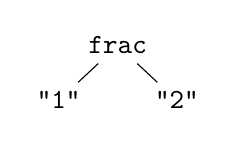
\begin{tikzpicture}[
            level 1/.style={sibling distance=15mm, level distance=7mm},
            every node/.style={align=center}
        ]
        \node {\texttt{frac}}
        child {node {\texttt{"1"}}}
        child {node {\texttt{"2"}}};
    \end{tikzpicture}
    \caption{The Tree Structure of \texttt{.tmu} Formulas}
    \label{fig:frac-tree}
\end{figure}

As a further example, consider the mathematical expression in Equation~\eqref{eq:tree-struc}:

\begin{equation}
    \label{eq:tree-struc}
    \int_{a}^{b} f(x) \, \mathrm{d}x = \left[ F(x) \right] \Big|_{a}^{b}
\end{equation}

% Its \texttt{.tmu} tree\footnote{On disk, a \texttt{.tmu} file stores this tree in an XML-like serialization; throughout this paper we display the same tree in the equivalent S-expression notation for readability, the two being interconvertible without information loss. Note that AI is sensitive to XML syntax~\cite{sui2024Table}, so the \texttt{.tmu} representation is conducive to the training and task performance of LLMs.} is shown in Listing~\ref{lst:scheme-integral}:
Its \texttt{.tmu} tree\footnote{On disk, a \texttt{.tmu} file stores this tree in an XML-like serialization; throughout this paper we display the same tree in the equivalent S-expression notation for readability, the two being interconvertible without information loss.} is shown in Listing~\ref{lst:scheme-integral}:
\begin{lstlisting}[caption={The \texttt{.tmu} tree of the integral, in S-expression notation},label={lst:scheme-integral},upquote=true]
> `(math (concat (big "int") (rsub "a") (rsup "b") "f" (around* "(" "x" ")") "<mathd>x=" (around* "<nobracket>" (around* "[" (concat "F" (around* "(" "x" ")")) "]") "|") (rsub "a") (rsup "b")))
\end{lstlisting}

Note that the segment $\left[ F(x) \right] |$ is managed via the tree structure illustrated in Figure~\ref{fig:tree-representation}. Consequently, even if a user omits a parenthesis or two, this omission does not negatively affect the rendering of the entire mathematical expression under the \texttt{.tmu} representation.

\begin{figure}[htbp]
    \vspace{-4mm}
    \centering
    \small
    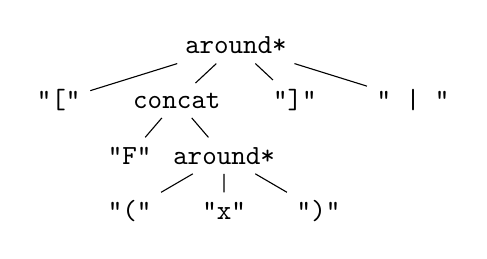
\begin{tikzpicture}[
            level 1/.style={sibling distance=15mm, level distance=7mm},
            level 2/.style={sibling distance=12mm, level distance=7mm},
            level 3/.style={sibling distance=12mm, level distance=7mm},
            every node/.style={align=center}
        ]
        \node {\texttt{around*}}
        child {node {\texttt{"["}}}
        child {node {\texttt{concat}}
                child {node {\texttt{"F"}}}
                child {node {\texttt{around*}}
                        child {node {\texttt{"("}}}
                        child {node {\texttt{"x"}}}
                        child {node {\texttt{")"}}}
                    }
            }
        child {node {\texttt{"]"}}}
        child {node {\texttt{" | "}}};
    \end{tikzpicture}
    \caption{Tree representation of $ [F (x)] |$}
    \label{fig:tree-representation}
\end{figure}

Unlike \TeX{}, this tree structure exists at the rendering level, not the syntax level. This rendering-level tree structure offers two distinct advantages:

\begin{enumerate}
    \item \textbf{Local Scoping of Input Errors:}
          \begin{itemize}
              \item Errors do not cause the entire document to fail rendering (a major drawback of \LaTeX{}).
              \item Local edits do not trigger global layout instability (a major drawback of MS Word).
          \end{itemize}

    \item \textbf{Independent Subtree Layout:} Because the document is represented as a tree, independent subtrees can be laid out separately rather than strictly serially, which can reduce the work required to re-render after a local edit.
\end{enumerate}

The same locality extends beyond formulas: each line, image block, and structural element maps to an independent tree node, so local edits such as resizing an image need not disrupt surrounding layout.
% Removed for page budget; keep source for possible restoration.
% We consider one further example. For a two-line layout like Figure~\ref{fig:double-line}, the representation is:
% \begin{lstlisting}
% > `(document "Logo" "(figure )" (itemize (document (concat (item) "WYSIWYG Writing") "")))
% \end{lstlisting}
%
% \begin{figure}[htbp]
%     \vspace{-4mm}
%     \centering
%     
\includegraphics[width=0.5\columnwidth]{figure/double-line.png}
%     \caption{Image insertion between lines}
%     \label{fig:double-line}
%     \vspace{-6mm}
% \end{figure}
%
% \begin{figure}[htbp]
%     \centering
%     \small
%     \begin{tikzpicture}[
%             level 1/.style={sibling distance=16mm, level distance=10mm},
%             level 2/.style={sibling distance=14mm, level distance=7mm},
%             every node/.style={
%                 align=center,
%                 text width=18mm
%             }
%         ]
%         \node {\texttt{document}}
%         child {node {``Logo''}}
%         child {node {\texttt{figure}}
%                 child {node {image}}
%             }
%         child {node {``WYSIWYG Writing''}};
%     \end{tikzpicture}
%     \caption{The \texttt{.tmu} multi-line data structure}
%     \label{fig:multiline-mogan}
%     \vspace{-4mm}
% \end{figure}
%
% This corresponds to the tree structure shown in Figure~\ref{fig:multiline-mogan}. As the figure demonstrates, in the \texttt{.tmu} representation, each line of content and every image block maps to an independent leaf node within the tree. Consequently, modifying an image (e.g., resizing or replacing it) need affect only that specific leaf node, without disrupting the layout of surrounding lines. This design effectively resolves the issue common in unstructured editors such as Word, where local modifications often lead to global layout chaos.

\subsection{Functional Symbol Representation}

In \TeX{}, all mathematical symbols and fonts are represented as strings. However, in the \texttt{.tmu} representation, certain special symbols are defined via functions. For instance, the inner product $\langle \cdot \rangle$, as shown in Equation~\eqref{eq:braket}, is an anonymous function that automatically scales according to the symbols it contains. While this is similar to \verb|\langle \rangle| in \LaTeX{}, the difference lies in the fact that, as a complete function, the left and right brackets always render a unified pair rather than isolated characters. To obtain a single bracket, a structured editor operating on \texttt{.tmu} lets the user delete the undesired character from the rendered pair.

\begin{equation}
    \label{eq:braket}
    \left\langle \int \right\rangle \langle f \rangle
\end{equation}

\subsection{Dynamic System Optimization}

The \texttt{.tmu} representation encodes citation relationships as structural links directly embedded in the document tree. This mechanism avoids a full re-parsing of the document when updating. Furthermore, because complexity is dictated by what the document tree actually contains, an editor operating on \texttt{.tmu} can load functionality on demand rather than relying on a pre-configured feature set, so that system complexity is dictated by document content. This mechanism significantly reduces the burden for deploying cloud environments or sandboxes. \emph{(Further details on reference rendering and plugin loading are available in Appendix~\ref{app:ren} and Appendix~\ref{app:plug}.)}
